\documentclass{include/thesisclass}
\usepackage{esvect}
\usepackage{amsthm}
\usepackage{listings}
% Main File - Based on thesisclass.cls
% Comments are mostly in English
% ------------------------------------------------------------------------------
% Further files in folder:
%  - include/cmds.tex (for macros and additional commands)
%  - include/kitlogo.pdf (for titlepage)
%  - lit.bib (bibtex bibliography database)
%  - include/titlepage.tex (for layout of titelpage)
% ------------------------------------------------------------------------------
% Useful Supplied Packages:
% amsmath, amssymb, mathtools, bbm, upgreek, nicefrac,
% siunitx, varioref, booktabs, graphicx, tikz, multicol





%% -------------------------
%% |    Thesis Settings    |
%% -------------------------
% english or ngerman (new german für neue deutsche Rechtschreibung statt german)
\SelectLanguage{ngerman}
% details on this thesis
\newcommand{\thesisauthor}{Kiril Voigtländer}
\newcommand{\thesistopic}{Name des Themas auf Deutsch}
\newcommand{\thesisentopic}{Name of the Topic in English}
\newcommand{\thesislongtopic}{Very long and very detailed description of the very interesting thesis topic (only necessary for pdfsubject tag).}
\newcommand{\thesisinstitute}{Otto-Kühne-Schule}
\newcommand{\thesisreviewerone}{Herr Schmalstieg}
\newcommand{\thesisreviewertwo}{}
\newcommand{\thesisadvisorone}{} % to use: enter names and uncomment in titlepg
\newcommand{\thesisadvisortwo}{}
\newcommand{\thesistimestart}{01.04.2015} % on titlepage
\newcommand{\thesistimeend}{30.09.2015} % on titlepage
\newcommand{\thesistimehandin}{30.09.2015} % on second page 'preamble'
\newcommand{\thesispagehead}{Facharbeit: \thesisentopic} % page heading





%% ---------------------
%% |    PDF - Setup    |
%% ---------------------
% This information will appear embed into the PDF file as meta data, but will 
% not be printed anywhere
\hypersetup
{
    pdfauthor={\thesisauthor},
    pdftitle={Bachelorarbeit: \thesistopic},
    pdfsubject={\thesislongtopic},
    pdfkeywords={kit,physik,bachelor,thesis,\thesisauthor}
}





%% --------------------------------------
%% |    Settings for Word Separation    |
%% --------------------------------------
% Help for separation:
% In German package the following hints are additionally available:
% "- = Additional separation
% "| = Suppress ligation and possible separation (e.g. Schaf"|fell)
% "~ = Hyphenation without separation (e.g. bergauf und "~ab)
% "= = Hyphenation with separation before and after
% "" = Separation without a hyphenation (e.g. und/""oder)

% Describe separation hints here:
\hyphenation
{
    über-nom-me-nen an-ge-ge-be-nen
    %Pro-to-koll-in-stan-zen
    %Ma-na-ge-ment  Netz-werk-ele-men-ten
    %Netz-werk Netz-werk-re-ser-vie-rung
    %Netz-werk-adap-ter Fein-ju-stier-ung
    %Da-ten-strom-spe-zi-fi-ka-tion Pa-ket-rumpf
    %Kon-troll-in-stanz
}





%% -----------------------
%% |    Main Document    |
%% -----------------------
\usepackage{lipsum} % for Lorem Ipsum text example
\begin{document}
    % Titlepage and ToC
    \FrontMatter

    % coordinates for background border
\newcommand{\diameter}{20}
\newcommand{\xone}{-15}
\newcommand{\xtwo}{160}
\newcommand{\yone}{15}
\newcommand{\ytwo}{-253}




\begin{titlepage}
    % background border
    \begin{tikzpicture}[overlay]
    \draw[color=gray]
            (\xone mm, \yone mm)
      -- (\xtwo mm, \yone mm)
    arc (90:0:\diameter pt)
      -- (\xtwo mm + \diameter pt , \ytwo mm)
        -- (\xone mm + \diameter pt , \ytwo mm)
    arc (270:180:\diameter pt)
        -- (\xone mm, \yone mm);
    \end{tikzpicture}



    % KIT image and sign for faculty of physics
    \begin{textblock}{10}[0,0](4.5,2)
         \includegraphics[width=.25\textwidth]{include/PädaLogo.pdf}
    \end{textblock}
    \changefont{phv}{m}{n}    % helvetica
    \begin{textblock}{10}[0,0](5.5,2.2)
        \begin{flushright}
            \Large Leistungskurs PHYSIK\\\thesisinstitute
        \end{flushright}
    \end{textblock}



    % horizontal line
    \begin{textblock}{10}[0,0](4.2,3.1)
        \begin{tikzpicture}[overlay]
        \draw[color=gray]
                (\xone mm + 5 mm, -12 mm)
          -- (\xtwo mm + \diameter pt - 5 mm, -12 mm);
        \end{tikzpicture}
    \end{textblock}



    % begin of text part
    \changefont{phv}{m}{n}    % helvetica
    \centering



    % thesis topic (en and ge)
    \vspace*{3cm}
    \Huge\thesistopic\\
    \huge(\thesisentopic)\\



    % author name and institute
    \vspace*{2cm}
    \Large Facharbeit\\von\\
    \vspace*{1cm}
    \huge\thesisauthor\\
    \vspace*{1cm}
    \Large an der \thesisinstitute



    % possible frontimage - thanks to JabberWok
    % for publishing the img under GNU Document License
    \vspace*{1.5cm}
    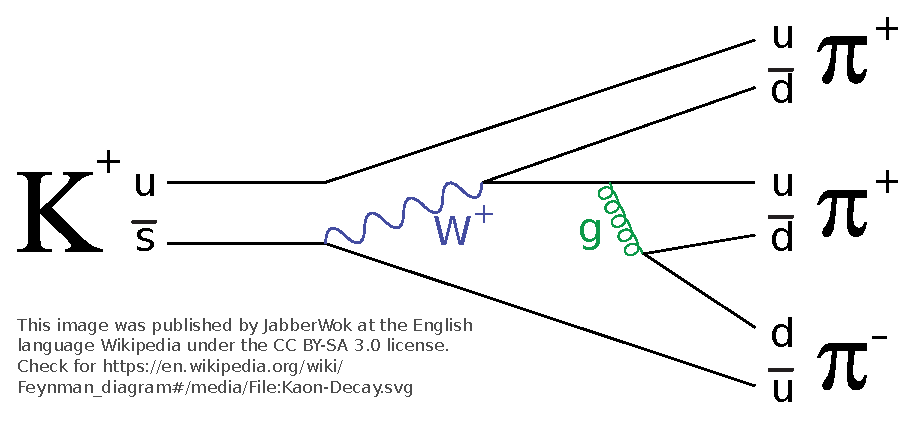
\includegraphics[scale=0.7]{./include/frontimage.eps}\\



    % examiners (Referenten)
    \vspace*{1.5cm}
    \Large
    \begin{center}
        \begin{tabular}[ht]{l c l}
        \iflanguage{english}{Reviewer}{Referent}: 
            & \hfill & \thesisreviewerone\\
        \iflanguage{english}{Second Reviewer}{Korreferent}: 
            & \hfill & \thesisreviewertwo\\
        % uncomment if you want to provide info on your advisors
        %\iflanguage{english}{Advisor}{Betreuender Mitarbeiter}: 
        %    & \hfill & \thesisadvisorone\\
        %\iflanguage{english}{Second Advisor}{Zweiter betreuender Mitarbeiter}: 
        %    & \hfill & \thesisadvisortwo\\
        \end{tabular}
    \end{center}



    % working time
    \vspace{1cm}
    \begin{center}
        \large{{Bearbeitungszeit}: \thesistimestart \hspace*{0.25cm} -- %
                                   \hspace*{0.25cm} \thesistimeend}
    \end{center}



    % lowest text blocks concerning the KIT
    \begin{textblock}{10}[0,0](4,16.8)
        \tiny{PÄDA -- Otto-Kühne-Schule}
    \end{textblock}
    \begin{textblock}{10}[0,0](14,16.75)
        \large{\textbf{www.kit.edu}}
    \end{textblock}
\end{titlepage}

    \chapter*{Erklärung zur Selbstständigkeit}
Ich versichere, dass ich diese Arbeit selbstständig verfasst habe und keine %
anderen als die angegebenen Quellen und Hilfsmittel benutzt habe, die %
wörtlich oder inhaltlich übernommenen Stellen als solche kenntlich gemacht habe. %und %
%die Satzung des KIT zur Sicherung guter wissenschaftlicher Praxis in der %
%gültigen Fassung vom 17.05.2010 beachtet habe.\\

\vspace{1cm}

\renewcommand{\arraystretch}{0} % for spacing in the tabular environment

\begin{flushright}
	\begin{tabular}{rr}
		Bonn, den \thesistimehandin, & \hspace*{5cm}\\[0mm]
		\cline{2-2}\\[2mm]    % the last line has height 2mm due
		& \thesisauthor       % to \arraystretch=0
	\end{tabular}
\end{flushright}

\vfill

\begin{flushright}
	Als Ansichtsexemplar genehmigt von\\
	\vspace{1cm}
	\begin{tabular}{rr}
		Bonn, den \thesistimehandin, & \hspace*{5cm}\\[0mm]
		\cline{2-2}\\[2mm]    % the last line has height 2mm due
		& \thesisreviewerone  % to \arraystretch=0
	\end{tabular}
\end{flushright}

\renewcommand{\arraystretch}{1}

%\cleardoublepage


    \begingroup \let\clearpage\relax    % in order to avoid listoffigures and
    \tableofcontents                    % listoftables on new pages
    \listoffigures
    \listoftables
    \endgroup
    \cleardoublepage



    % Contents
    \MainMatter

    \chapter{Introduction}
    Die vorliegende Facharbeit befasst sich mit dem Modell des Röhrenfernsehrs.
Röhrenfernsehr sind Geräte bei welchem ein Bild durch entweder einer elektrischen oder einer magnetischen Ablenkung auf einen Bildschirm gelenkt werden.
Des Weiteren wird der Röhrenfernsehr in der dazu gelegten Animation bildlich dargestellt.
Sowohl die Animation als auch ihre physikalischen Eigenschaften werden in dem Kapitel \ref{chap:sim} erläutert.
Im ersten Kapitel nach der Einleitung wird die Theorie des E-Feldes und des B-Feldes betrachtet.
Für das E-Feld wichtig ist, dass es eine Ladung gibt, da um jede Ladung ein elektrisches Feld gibt.
Des Weiteren wird die Herleitung der Coulombkraft betrachtet.
Anschließend folgt eine genauere Betrachtung eines Plattenkondensators, welcher einen Spezialfall eines elektrischen Feldes darstellt.
Dabei wird auf die Formel für die Kapazität "`$C$"' und für die gespeicherte Energie im Plattenkondensator betrachtet.
Dies geschieht im Kapitel \ref{sec:Plattenkondensator}.
Für das B-Feld ist der Magnetismus wichtig, welcher zu der Entstehung des B-Feldes führt.
Hier wird die Herleitung der Lorentzkraft getätigt.
Anschließend folgt eine genauere Betrachtung des Fadenstrahlrohrs, welcher zur der Bestimmung der spezifischen Ladung "`$\frac{e}{m}$"' benutzt wird.
Diese Betrachtung geschieht im Kapitel \ref{sec:Fadenstrahlrohr}.
Des Weiteren wird die Wechselwirkung der beiden Felder aufeinander betrachtet.
%genauer erklären was passiert. geht erst nach der stunde mit dem tutor und nachdem schreiben des Kapitels
Dies geschieht im Kapitel \ref{sec:Maxwell}.
Das folgende Kapitel \ref{chap:fern} ist in zwei unter Teile aufgeteilt.
Im ersten Unterteil \ref{sec:aufbau} wird der Aufbau der Fernsehröhre betrachtet.
Dabei ist wichtig zu beachten, dass ein Röhrenfernsehr aus einer Einrichtung besteht, welche die Elektronen emittiert, einer Einrichtung, welche die Elektronen steuert, eine Einrichtung, welche die Elektronen ablenkt und einen Bildschirm, wo die Elektronen als Strahl auf einen Punkt treffen, wo das Bild erzeugt wird.
Die Ablenkung kann sowohl magnetisch als auch elektrisch sein.
Die Funktionsweise der Fernsehröhre wird im Kapitel \ref{sec:Funktionsweise} behandelt.
In diesem Kapitel wird des weiteren auch erklärt, welche Kräfte auf das jeweilige Elektron in der jeweiligen Einrichtung wirken und welche Resultate dies mit sich zieht.

    \chapter{Theoretical Background}
    \section{E-Feld:}
\subsection{Entstehung und Beschreibung}
Jede Ladung wird von einem elektrischen Feld umgeben.
Zuerst muss der Begriff von Ladung geklärt werden:
Ladung ist eine Eigenschaft von Materie.
Die Einheit der Ladung ist 1$C$ (Coulomb).
Alle bisherigen Experimente legen nahe, dass es nur 2 Arten von elektrischer Ladung gibt; Positiv und Negativ.
Die Richtung der Feldlinien ist immer die Richtung der Kraftwirkung auf einen positiv geladenen Probekörper.
Eine Ladung bewirkt eine Kraft auf eine andere Ladung.
Gleich geladene Ladungen stoßen sich ab, während entgegengesetzte geladene Ladungen sich anziehen.
Diese Kraft wird als elektrische Kraft bezeichnet oder genauer als Coulomb-Kraft.
Die Herleitung der Coulomb-Kraft sieht wie folgt aus:
Man nehme sich zwei Punktladungen, welche mit $q_1$ und mit $q_2$ gekennzeichnet werden. 
Des Weiteren ist ein Abstand $r$ zwischen den Ladungen vorhanden.
Es gibt einmal die Kraft von $q_1$ auf $q_2$ ($\vv{F_{12}}$) und einmal die Kraft von $q_2$ auf $q_1$ ($\vv{F_{21}}$).
Durch betrachten der Formel: $F_{el} = \frac{q_1 \cdot q_2}{r^2}$ 
lässt sich schließen, dass wenn $r$ gleich bleibt, aber die die Ladungen $q_1$ und $q_2$ erhöht werden, die Coulomb-Kraft ebenfalls zunimmt.
Daraus lässt sich schließen, dass die elektrische Kraft proportional zu den Ladungen $q_1$ und $q_2$ ist. 
Wenn die Ladungen $q_1$ und $q_2$ gleich bleiben und $r$ erhöht wird, dann verringert sich die elektrische Kraft.
Daraus lässt sich wiederum schließen, dass die elektrische Kraft anti proportional zum Abstand $r$ ist.
Diese zuvor beschriebene Kraftwirkung, lässt sich mittels Probeladungen im ganzen Raum um die Ladung messen und als Vektor an jedem Punkt visualisieren.
Diese Visualisierung des Raumes nennt man elektrisches Feld.
Die jeweilige Stärke ergibt sich aus der Größe der Probeladung "`$q$"' und der Größe der Kraft "`$F_{el}$"' auf die Ladung.
Die Formel für das E-Feld ist : $E = \frac{F_{el}}{q}$.
Die Dimension des E-Feldes lautet: $[E] = \frac{N}{C} = \frac{V}{m}$.
Veranschaulichen lässt sich dies durch die Animation \cite{Animation}.

%Beschreibung
Wenn ein elektrisches Feld vorhanden ist, lässt sich dieses als Eigenschaft des Raums auffassen.
Die Kraftwirkung des elektrischen Feldes wird mit Probeladung ermittelt und durch Feldlinien visuell dargestellt.
Die Feldlinien kreuzen und berühren sich nicht.
Wenn die Feldlinien eng beieinander liegen (hohe Dichte), dann ist das dort existierende elektrische Feld stark.
Wenn die Dichte der Feldlinien allerdings niedrig ist, dann ist das elektrische Feld schwach.
Es gibt zwei unterschiedliche Arten von elektrischen Feldern. 
Es gibt zum einen das homogene elektrische Feld und zum anderen das inhomogene elektrische Feld.
Bei dem homogenen elektrischen Feld stehen die Feldlinien parallel zu einander und das elektrische Feld ist an allen Stellen gleich stark.
Bei dem inhomogenen elektrischen Feld kann diese Annahme nicht getätigt werden.
% hier eventuell noch auf die verschiedene Ladungen eingehen (Punktladung, etc.)
\subsection{Anwendung}
Als Anwendungsbeispiel lässt sich der Plattenkondensator nehmen:
Hier lässt sich die Annahme treffen, dass das elektrische Feld zwischen den Platten homogen ist.
Des Weiteren ist das elektrische Feld als $E = \frac{U}{d}$ definiert.
Somit nimmt das elektrische bei einer größeren Spannung "`U"' zu und bei größerem Abstand der Platten "`d"' ab.
Beim Kondensator kann noch eine weitere Größe eingeführt werden, die Kapazität "`C"'.
Die Kapazität ist dabei so definiert, dass sie die maximale Menge an Ladung, die der Kondensator auf den Platten speichern kann, angibt.
Die Herleitung ist wie folgt:
$\mbox{Flächenladungsdichte: } \sigma \mbox{:=} \frac{Q}{A}$.
Dies führt zum elektrischen Feld mit $\sigma = \epsilon_0 \cdot E$ als Feldgleichung.
Dabei beträgt $\epsilon_0 = 8.854 \cdot 10^{-12} \frac{As}{Vm}$ und ist unter dem Namen "`Dielektrizitätskonstante"' bekannt.
Im allgemeinen ist das Feld auch noch vom jeweiligen Material abhängig, wodurch die Gleichung einen weiteren Term "`$\epsilon_r$"'enthält "`$\sigma = \epsilon_0 \cdot \epsilon_r \cdot E$ "'.
Diese zusätzliche Konstante berücksichtigt dabei die spezifische Materialeigenschaften und nennt sich "` relative Permeabilität"'.
Im Vakuum ist diese jedoch = 1.
Daraus folgt, dass $ Q = \epsilon_0 \cdot \epsilon_r \cdot \frac{A}{d} \cdot U$ ist.
Die Kapazität ist als $\mbox{C:= } \frac{Q}{U} = \epsilon_0 \cdot \epsilon_r \cdot \frac{A}{d}$ definiert.
Des Weiteren kann die Energie im Plattenkondensator bestimmt werden.
Dafür wird angenommen, dass der Kondensator zuerst neutral ist und eine äußere Spannung $U_0$ anliegt.
Im ersten Schritt fließt eine kleine Portion Ladung $\Delta Q$ mit dem Energieaufwand $\Delta W_1$ auf die andere Platte. Dabei entsteht die Spannung $U_1$ zwischen den Platten $\rightarrow$ $\Delta W_1 = U_1 \cdot \Delta Q$.
Es wird mehr Energie benötigt, um  weitere gleichgroße Ladungsportionen $\Delta Q$ auf die Platte zu bringen $\Delta W_2 = U_2 \cdot \Delta Q$.
Die letzte Ladungsportion $\Delta Q$ wird mit der Energie $\Delta W_E$ auf die Platte transportiert und dabei liegt zwischen den Platten die Spannung $U_0$ an. 
$\Delta W_E = U_0 \cdot \Delta Q$.
Daraus folgt die Gesamtenergie: W = $\Delta W_1 + \Delta W_2 +...+ \Delta W_E$
$$\Rightarrow W \mbox{ = } \frac{1}{2}\cdot Q_E \cdot U_o \mbox{ wegen $Q_E = C \cdot U_0$}$$
$$W= \frac{1}{2} \cdot C \cdot U_o^2$$
\section{B-Feld:}
\subsection{Entstehung und Beschreibung}
Als Grundlage, dass ein B-Feld entsteht muss der Magnetismus als Grundlage genommen werden.
Dafür muss der Begriff des Magnetismus zu erst geklärt werden.
Ein Magnet wird dadurch Entmagnetisiert, dass er gestoßen oder mit einer Temperatur oberhalb der Curie-Temperatur erhitzt wird $~600°C$.
Des Weiteren führt das Durchbrechen eines Magneten in der Mitte, dazu das zwei neue Magneten entstehen, es gibt keine magnetische Monopole.
Die Feldlinien eines Magneten verlaufen vom Nordpol zum Südpol.
Ein Magnetfeld bewirkt eine Kraft auf ein geladenes Teilchen.
Die wirkende Kraft wird als magnetische Kraft bezeichnet oder als Lorentzkraft, wenn es sich um einen einzelnen Ladungsträger handelt.
Die Herleitung der Lorentzkraft sieht wie folgt aus:
Man nehme sich einen Ladungsträger (negativ) und einen langen Leiter.
Die Formel für die magnetische Kraft lautet: $F_{mag} =  B \cdot I_L \cdot \Delta l$.
Der Strom $I_L$ kann durch $\frac{\Delta Q}{\Delta t}$ ersetzt werden.
Dadurch kommt die Formel $F_{mag} = B \cdot \frac{\Delta Q}{\Delta t} \cdot l$ raus. 
Als nächstes lässt sich $\Delta Q$ durch $N \cdot e$ ersetzten.
Dies führt zu der Formel $F_{mag} = B \cdot N \cdot e \cdot \frac{\Delta l}{\Delta t}$.
Dabei lässt sich der Quotient als $v$ vereinfachen, was die Geschwindigkeit der Ladungsträger angibt.
Dadurch beträgt die Formel für die magnetische Kraft nun: $F_{mag} = B \cdot N \cdot e \cdot v$.
Allerdings soll die Lorentzkraft hergeleitet werden, welches die Kraft auf einen einzelnen Ladungsträger darstellt, weshalb die magnetische Kraft mit $N$ dividiert werden muss.
Dies führt dazu, dass die Formel für die Lorentzkraft $F_L = B \cdot e \cdot v$ ist.
Diese Formel lässt sich für jede beliebige Ladung benutzen, weshalb $e$ durch $q$ ersetzt werden kann.
Daraus ergibt sich die Formel: $F_L = q \cdot B \cdot v$.
Der Vektor der Lorentzkraft senkrecht auf der durch den Geschwindigkeitsvektor und dem Vektor der Flussdichte aufgespannten Ebene \cite{Lorentzkraft}.
Magnetfelder entstehen in der Gegenwart von Dauermagneten (bestehend aus Eisen, Kobalt, Nickel oder Legierungen) oder in der Umgebung von stromdurchflossenen Leitern. 
Die Größe der magnetischen Flussdichte "`B"' ist den magnetischen Feldlinien zugeordnet.
Sie ist durch die Kraft definiert, welche ein stromdurchflossener Leiter erfährt.
Die Visualisierung des Raums nennt man magnetisches Feld.
Die jeweilige Stärke ergibt sich aus der Größe der Kraft "`$F_L$"', der Länge des Leiters "`$l$"' und der Stärke des elektrischen Stroms "`$I$"'.
Die Formel für das B-Feldd ist : $B = \frac{F_L}{I \cdot l}$.
Die Dimension des B-Feldes lautet: $[B] = \frac{N}{Am} = \frac{Vs}{m^2} = T$.

% Beschreibung von B-Feld
Wenn ein magnetisches Feld vorhanden ist, lässt sich dieses als Eigenschaft des Raums auffassen.
Die Kraftwirkung des magnetischen Feldes wird durch geladen Teilchen (Ladungen) ermittelt und durch Feldlinien visuell dargestellt.
Die Feldlinien kreuzen und berühren sich nicht.
Des Weiteren haben Sie keinen Anfangspunkt und kein Endpunkt, sondern sind stets geschlossen.
Wenn die Dichte an Feldlinien groß ist, dann ist die Magnetfeldstärke dementsprechend ebenfalls stark.
Wenn die Dichte an Feldlinien gering ist, dann ist die Magnetfeldstärke ebenfalls gering.
Es gibt verschiedene Magnete mit dementsprechend auch verschiedene Magnetfeldern. 
Zum einen liegt der Stabmagnet vor, bei welchem das magnetische Feld analog zum elektrischen Feld eines Dipols ist.
Zum anderen liegt der Hufeisenmagnet vor, welcher gleich wie der Plattenkondensator abgebaut ist.
Bei diesem ist das magnetische Feld im inneren homogen und an den Rändern inhomogen. 
\subsection{Anwendung}

\section{Wechselwirkung der Felder}%Maxwellgleichung
    \chapter{Experimental Investigations}
    \section{Experimenteller Aufbau}

\paragraph{meine Einstellungsparameter:}

\begin{itemize}
    \item Beschleunigungsspannung $U_B$ im Bereich von 12 kV bis 16 kV, zugehöriger Richtungsvektor $\vv{s} = \vektor{1}{0}{0}$
    \item Magnetfeldstärke zweier Ablenkspulen:
    
    \begin{itemize}
        \item $B_1$ im Bereich -5 mT bis 5 mT, zugehöriger Richtungsvektor $\vv{b_1} = \vektor{0}{0}{1}$ % senkrechte Spule
        \item $B_2$ im Bereich -5 mT bis 5 mT, zugehöriger Richtungsvektor $\vv{b_2} = \vektor{0}{1}{0}$ % waagerechte Spule
    \end{itemize}

\end{itemize}

\paragraph{Konstanten:}

\begin{itemize}
    \item Felddurchmesser $d$ = 30 in mm
    \item Masse des Elektrons $m$ =  $9,109 \cdot 10^{-31}$ in kg
    \item Ladung des Elektrons $e$ = $1,602 \cdot 10^{-19}$ in As
    \item Bildschirmabstand $l$ = 500 in mm
\end{itemize}

\paragraph{meine zu berechnenden Parameter:}

\begin{itemize}
    \item Teilchengeschwindigkeit v in $\frac{km}{s}$
    \item Ergebnisvektor $\vv{v}$
    \item Bahnradius r in mm 
    \item alpha $\alpha$
    \item Ablenkungsrichtung $\vv{a}$
\end{itemize}

\section{Berechnung der Elektronenkanone}
Das ist im Strahl und hier wird die Geschwindigkeit berechnet mit welcher dieser aus der Elektronenkanone kommt. 

\subsection{physikalische Erklärung:}

Durch den glühelektrischen Effekt werden Elektronen freigesetzt. Dabei wird ein "Wehnelt-Zylinder" durch eine Heizspannung $U_H$ erhitzt. Die nun freien Elektronen werden durch die Kathode (positiver Pol) gebündelt. Dies geschieht dadurch das in der Mitte der Platte ein kleines Loch vorhanden ist durch welches der Elektronenstrahl nun fließt. Um die Geschwindigkeit zu bestimmen muss der Energieerhaltungssatz betrachtet werden. Dabei wird die kinetische Energie und die elektrische Energie gleichgesetzt. Um die elektrische Energie benutzen zu können, wird das Ende des "Wehnelt-Zylinder" als Anode aufgefasst( negativer Pol) und dadurch entsteht ein elektrisches Feld in welchem auch die elektrische Energie vorhanden ist. 
$$ E_{kin} = E_{el}$$
$$ \frac{1}{2} \cdot m \cdot v^2 = e \cdot U_B$$
Diese Formel wird  nun nach v umgestellt:
\subsection{Die physikalische Formel:} 
$$ v = \sqrt{\frac{2 \cdot e \cdot U_B}{m}}$$

\subsection{Erklärung/Umsetzung der Physik im Code:}

Im Folgenden ist der Code in der Simulation dargestellt. Zu sehen ist, dass die oben genannte Formel benutzt wird und die jeweiligen Attribute aus den zugehörigen Klassen geholt werden. Hier muss sich die Spannung $U_B$ aus der Elektronenkanone (\lstinline$quelle$)  geholt werden. Des Weiteren wird die Spannung mit 1000 multipliziert, da in der Formel mit V gerechnet wird, während die Spannung der Elektronenkanone in kV angegeben ist. Deswegen muss diese noch umgerechnet werden.
\begin{lstlisting}
teilchengeschwindigkeit 
  = Math.sqrt(2 
  * elektronenladung 
  * quelle.spannung 
  * 1000 
  / elektronenmasse);
\end{lstlisting}

\section{Lorentzkraft und Ablenkung}

Das ist im Magneten und hier wird die Ablenkung berechnet.


\subsection{physikalische Erklärung:}
Das Magnetfeld der Ablenkspulenpaare ist homogen und steht senkrecht zu der Bewegungsrichtung der Elektronen. Die Elektronen kommen mit einer gewissen Geschwindigkeit $v$ aus der Elektronenkanone heraus und diese bleibt auch im weiteren Verlauf konstant. Dies bedeutet, dass die Lorentzkraft $F_L$ stets senkrecht zur Bewegungsrichtung der Elektronen wirkt und ihr Betrag dadurch konstant bleibt. Dies bedeutet, dass Sie deswegen als Zentripetalkraft auf die Elektronen wird und diese dadurch auf eine Kreisbahn zwingt. Wie bereits beschrieben, wirkt die Lorentzkraft als Zentripetalkraft immer senkrecht auf die Bewegungsrichtung der Elektronen. Dies bedeutet, dass die Kraftkomponente in Bewegungsrichtung nicht vorhanden ist und die Geschwindigkeit deswegen konstant bleibt. Dadurch leitet sich ab: 
$$ F_L=F_z$$
$$ e \cdot v \cdot B = \frac{m \cdot v^2}{r}$$
Dies lässt sich nun nach $r$ umstellen und man erhält die Formel \ref{eq:r}.   

\subsection{Die physikalische Formel:}

\begin{equation}
     \label{eq:r}
     r = \frac{m \cdot v}{e \cdot B}
\end{equation}


\subsection{Erklärung/Umsetzung der Physik im Code:}

Im Folgenden ist der Code in der Simulation dargestellt. Hier wird zuerst ebenfalls der \lstinline$Bahnradius$ berechnet, dies geschieht dadurch, dass die Elektronenmasse und die zuvor berechnete Teilchengeschwindigkeit mit aus dem Strahl geholt werden und miteinander multipliziert werden. Des Weiteren wird dieses Ergebnis durch die Elektronenladung und der Magnetfeldstärke mal 1000 dividiert. Die Elektronenladung wird sich ein weiteres mal aus der Klasse Strahl geholt, wo sie gespeichert wurde.
\begin{lstlisting}
bahnradius
  = strahl.elektronenmasse
    * strahl.teilchengeschwindigkeit
    / (strahl.elektronenladung * magnetfeldstaerke/1000)
    * 1000;
\end{lstlisting}

\section{Geometrische Bestimmung des Winkels}

Hier wird der Punkt auf dem Bildschirm berechnet.
\subsection{geometrische Erklärung:}
Um geometrisch die Ablenkung zu berechnen muss die Annahme getroffen werden, dass die Ablenkung des Magnetfeldes nur in einem kreisförmigen Ausschnitt wirkt. Die Situation ist wie in der Skizze in der Abbildung \ref{fig:ausBlog}.\footnote{Diese Abbildung wurde übernommen aus \url{https://www.physikerboard.de/ptopic,342494.html#342494}.} Aus der Skizze ergibt sich, dass der Ablenkwinkel, um den der Strahl geknickt wird, gleich ist zu dem Winkel im großen Kreis zwischen den Punkten A (Eintrittspunkt in den kleinen Kreis) und B (Austrittspunkt aus dem kleinen Kreis). Im rechtwinkligen Dreieck aus dem Punkt A und den beiden Mittelpunkten der Kreise, kann man die Definition des Tangens benutzen. Der Winkel ist $\frac{\alpha}{2}$ da die Winkelhalbierende als Verbindungslinie fungiert. Also gilt die Formel \ref{eq:tan}. Um festzustellen in welche Richtung um den Winkel $\alpha$ abgelenkt wird, müssen die Richtungsvektoren des Strahls und des Magnetfeldes betrachtet werden. Die Lorentzkraft wirkt in die Richtung des Kreuzprodukts dieser beiden. Da mit negativen Teilchen gearbeitet wird, muss der Richtungsvektor des Strahls umgedreht werden. Dadurch ergibt sich die Formel \ref{eq:a}. 
\begin{figure}
    \centering
    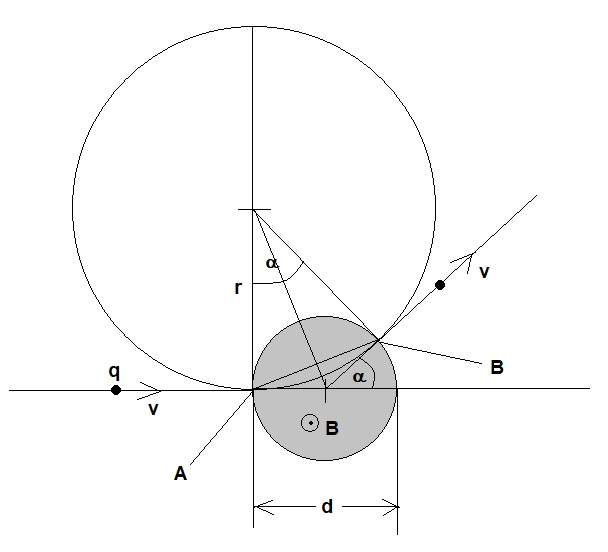
\includegraphics[width=.75\textwidth]{fig/elektronenstrahl-ablenkung_101.jpg}
    \caption{Skizze für Winkelberechnung}
    \label{fig:ausBlog}
\end{figure}

\subsection{Die geometrische Formel:}
\begin{equation}
    \label{eq:tan}
    \tan(\frac{\alpha}{2}) = \frac{d}{2}:r = \frac{d}{2 \cdot r}
\end{equation}

\begin{equation}
    \label{eq:a}
    \vv{a} = \vv{s} \cdot (-1) \times \vv{b}
\end{equation}

\begin{equation}
    \label{eq:v}
    \vv{v} = \vv{v} + \vv{a} \cdot l \cdot \tan(\alpha)
\end{equation}

\subsection{Erklärung/Umsetzung der Physik im Code:}
 Bei der Berechnung des Winkels $\alpha$ wird die oben %Verweis möglich?
bereits genannte Formel mit zwei multipliziert da auf der Ausgabe der tatsächliche Winkel $\alpha$ zu sehen sein soll. Des Winkel $\alpha$ wird im Bogenmaß berechnet. Bei der \lstinline$Ablenkungsrichtung$ wird der Richtungsvektor des Strahl mit $-1$ multipliziert und danach das Kreuzprodukt mit dem Richtungsvektor des Ablenkspulenpaars genommen. Durch den Befehl \lstinline$this.richtungsvektor$ wird auf den Richtungsvektor des jeweiligen Magnetes verwiesen. Des Weiteren ist noch hinzuzufügen, dass die Berechnung jedes Ablenkspulenpaar für sich macht uns daher auch eigene Werte für \lstinline$alpha$, den \lstinline$Bahnradius$ und die \lstinline$Ablenkungsrichtung$ hat.
\begin{lstlisting}
alpha = 2 * Math.atan(felddurchmesser/ (2 *bahnradius ));
ablenkungsrichtung
  = strahl.quelle.richtungsvektor.
    multiplizieren(-1).
    kreuzprodukt(this.richtungsvektor);

Vektor ergebnisvektor = new Vektor(bildschirmabstand,0,0);
    for(Ablenkspulenpaar m : getWorld().getObjects(Ablenkspulenpaar.class) )
    {
        ergebnisvektor 
        = ergebnisvektor.addieren( m.ablenkungsrichtung.
        multiplizieren(bildschirmabstand).
        multiplizieren(Math.tan(m.alpha)));
    }
return ergebnisvektor;

\end{lstlisting}

\begin{tabular}{c|c|c}
     Formel Buch & Formel Block & Anmerkungen  \\
     \hline
    $\alpha = \frac{d}{r}$ &$\tan(\frac{\alpha}{2}) = \frac{d}{2\cdot r}$& wegen Kleinwinkelnäherung bei dem Buch \\
    \hline
   $r = \frac{m\cdot v}{q\cdot B}$  & $r = \frac{m\cdot v}{q\cdot B}$& alles gleich 
     
\end{tabular}













 


    \emptychapter[3]{ROOT Routines}     % usage: \emptychapter[page displayed 
                                        %        in toc]{name of the chapter}



    \chapter{Conclusions}
    \section{\textbf{Graphische Ausarbeitung}}

Wenn immer man ein Objekt(Fernsehröhre oder jedes andere mögliche Objekt) auf einen Bildschirm abbilden möchte, muss man aus 3D in der "Realität" 2D auf dem Bildschirm machen. Dafür muss man eine Koordinatentransformation machen, welche auch als Kameratransformation bekannt ist.

\underline{Würfel:}
$$(x -100 \mbox{bis}  100)$$
$$(y-100\mbox{bis}100)$$
$$(z-100\mbox{bis}100$$

\underline{N Nullpunkt auf dem Schirm}
$$x = -60$$
$$y = -50$$
$$z = 30$$
\underline{a = Blickrichtung}
$$x = \sqrt{1/6}$$
$$y = \sqrt{2/3}$$
$$z = -\sqrt{1/6}$$
x, y sollen positiv sein, z soll negativ sein und der Betrag/Länge soll eins sein. X etwas kleiner als y.
$$y= \sqrt{2/3}$$
$$x= \sqrt{1/6}$$
\underline{b:}
z = 0 ; andere Werte so wählen, dass Skalarprodukt 0 ergibt
$$x= \sqrt{2/3}$$
$$y=-\sqrt{1/6}$$
$$z=0$$
$$|\vv{b}| = \sqrt{5/6} =/1 ; also müssen x und y mit dem Kehrwert von\sqrt{5/6} also mit \sqrt{6/5} multipliziert werden.$$

    % appendix for more or less interesting calculations
    \Appendix
    \chapter*{\appendixname} \addcontentsline{toc}{chapter}{\appendixname}
    % to make the appendix appear in ToC without number. \appendixname = 
    % Appendix or Anhang (depending on chosen language)
    \section{First Appendix Section}
Wonderful Appendix!

\lipsum[1-5]
 %\cleardoublepage



    % Bibliography
    \TheBibliography

    % BIBTEX
    % use if you want citations to appear even if they are not referenced to: 
    % \nocite{*} or maybe \nocite{Kon64,And59} for specific entries
    %\nocite{*}
    \bibliographystyle{babalpha}
    \bibliography{lit.bib}

    % THEBIBLIOGRAPHY
    %\begin{thebibliography}{000}
    %    \bibitem{ident}Entry into Bibliography.
    %\end{thebibliography}
\end{document}
